\chapter{The Derivative} \label{der:chapter}

%%%%%%%%%%%%%%%%%%%%%%%%%%%%%%%%%%%%%%%%%%%%%%%%%%%%%%%%%%%%%%%%%%%%%%%%%%%%%%

\section{The derivative}
\label{sec:der}

\sectionnotes{1 lecture}

The idea of a derivative is the following.
Let us suppose a graph of a function looks locally like a straight line.
We can then talk about the slope of this line.  The slope tells us 
the rate at which 
the value of the function changing at the particular point.
Of course, we are leaving out any function that has corners or
discontinuities.  Let us be precise.

\subsection{Definition and basic properties}

\begin{defn}
Let $I$ be an interval, let
$f \colon I \to \R$ be a function, and let $c \in I$.  If 
the limit
\begin{equation*}
L := \lim_{x \to c} \frac{f(x)-f(c)}{x-c} 
\end{equation*}
exists, then we say $f$ is
\emph{\myindex{differentiable}}\index{function!differentiable} at
$c$, that $L$ is the \emph{\myindex{derivative}} of $f$ at $c$,
and write $f'(c) := L$.\glsadd{not:derivative}

\medskip

If $f$ is differentiable at all $c \in I$, then we simply say that
$f$ is \emph{differentiable}, and then we obtain a function
$f' \colon I \to \R$.
The derivative is sometimes written as $\frac{df}{dx}$ or
$\frac{d}{dx}\bigl( f(x) \bigr)$.

\medskip

The expression $\frac{f(x)-f(c)}{x-c}$ is called the
\emph{\myindex{difference quotient}}.
\end{defn}

The graphical interpretation of the derivative is  depicted in
\figureref{derivfig}.  The left-hand plot gives the line through
$\bigl(c,f(c)\bigr)$
and $\bigl(x,f(x)\bigr)$ with slope
$\frac{f(x)-f(c)}{x-c}$, that is,
the so-called \emph{\myindex{secant line}}.  When we take the limit as $x$ goes to $c$,
we get the right-hand plot, where we see
that the derivative of the function
at the point $c$ is the slope of the line tangent to the graph of $f$
at the point $\bigl(c,f(c)\bigr)$.

\begin{myfigureht}
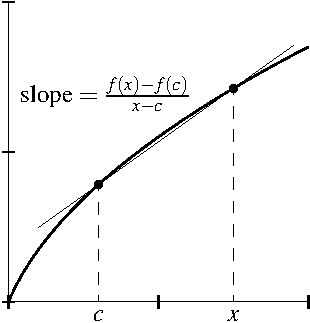
\includegraphics{figures/derivdfig}
\qquad
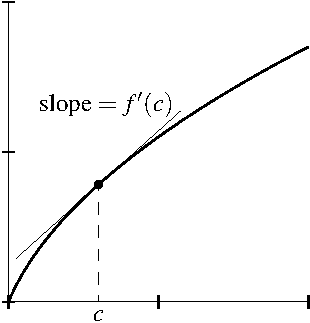
\includegraphics{figures/derivfig}
\caption{Graphical interpretation of the derivative.\label{derivfig}}
\end{myfigureht}

We allow $I$ to be a closed interval and we allow
$c$ to be an endpoint of $I$.  Some calculus books do not allow $c$ to be an
endpoint of an interval, but all the theory still works by allowing it, and
it makes our work easier.

\begin{example}
Let $f(x) := x^2$ defined on the whole real line.  Let $c \in \R$ be arbitrary.  We find that if
$x \not=c$,
\begin{equation*}
\frac{x^2-c^2}{x-c} =
\frac{(x+c)(x-c)}{x-c} =
(x+c) .
\end{equation*}
Therefore,
\begin{equation*}
f'(c) = 
\lim_{x\to c} \frac{x^2-c^2}{x-c} =
\lim_{x\to c} (x+c) = 2c.
\end{equation*}
\end{example}

\begin{example}
Let $f(x) := ax + b$ for numbers $a, b \in \R$.
Let $c \in \R$ be arbitrary.
For $x \not=c$,
\begin{equation*}
\frac{f(x)-f(c)}{x-c} =
\frac{a(x-c)}{x-c} = a .
\end{equation*}
Therefore,
\begin{equation*}
f'(c) =
\lim_{x\to c} 
\frac{f(x)-f(c)}{x-c} =
\lim_{x\to c} 
a = a.
\end{equation*}
In fact, every differentiable function ``infinitesimally'' behaves like
the affine function $ax + b$.  You can guess many results
and formulas for derivatives, if you work them out for affine functions
first.
\end{example}

\begin{example}
The function $f(x) := \sqrt{x}$ is differentiable for $x > 0$.  To see this
fact, fix $c > 0$,
and take $x \not= c$, $x > 0$.  Compute
\begin{equation*}
\frac{\sqrt{x}-\sqrt{c}}{x-c}
=
\frac{\sqrt{x}-\sqrt{c}}{(\sqrt{x}-\sqrt{c})(\sqrt{x}+\sqrt{c})}
=
\frac{1}{\sqrt{x}+\sqrt{c}} .
\end{equation*}
Therefore,
\begin{equation*}
f'(c) =
\lim_{x\to c}
\frac{\sqrt{x}-\sqrt{c}}{x-c}
=
\lim_{x\to c}
\frac{1}{\sqrt{x}+\sqrt{c}}
=
\frac{1}{2\sqrt{c}} .
\end{equation*}
\end{example}

\begin{example}
The function $f(x) := \abs{x}$ is not differentiable
at the origin.  When $x > 0$, then
\begin{equation*}
\frac{\abs{x}-\abs{0}}{x-0} =
\frac{x-0}{x-0} = 1 ,
\end{equation*}
and when $x < 0$ we have
\begin{equation*}
\frac{\abs{x}-\abs{0}}{x-0} =
\frac{-x-0}{x-0} = -1 .
\end{equation*}
\end{example}

A famous example of Weierstrass shows that there exists a continuous
function that is not differentiable at \emph{any} point.  The construction
of this function is beyond the scope of this book.  On the other hand,
a differentiable function
is always continuous.

\begin{prop}
Let $f \colon I \to \R$ be differentiable at $c \in I$,
then it is continuous at $c$.
\end{prop}

\begin{proof}
We know the limits
\begin{equation*}
\lim_{x\to c}\frac{f(x)-f(c)}{x-c} = f'(c)
\qquad
\text{and}
\qquad
\lim_{x\to c}(x-c) = 0
\end{equation*}
exist.  Furthermore,
\begin{equation*}
f(x)-f(c) = 
\left( \frac{f(x)-f(c)}{x-c} \right) (x-c) .
\end{equation*}
Therefore the limit of $f(x)-f(c)$ exists and
\begin{equation*}
\lim_{x\to c} \bigl( f(x)-f(c) \bigr) =
\left(\lim_{x\to c} \frac{f(x)-f(c)}{x-c} \right)
\left(\lim_{x\to c} (x-c) \right) =
f'(c) \cdot 0  = 0.
\end{equation*}
Hence $\lim\limits_{x\to c} f(x) = f(c)$, and $f$ is continuous at $c$.
\end{proof}

An important property of the derivative is linearity.  The
derivative is the approximation of a function by a straight line.
The slope of a line through two points changes linearly when the
$y$-coordinates are changed linearly.  By taking the limit,
it makes sense that the derivative is linear.

\begin{prop}
\index{linearity of the derivative}
Let $I$ be an interval, let
$f \colon I \to \R$ and $g \colon I \to \R$ be differentiable at $c \in I$,
and let $\alpha \in \R$.
\begin{enumerate}[(i)]
\item
Define $h \colon I \to \R$ by $h(x) := \alpha f(x)$.  Then
$h$ is differentiable at $c$ and
$h'(c) = \alpha f'(c)$.
\item
Define $h \colon I \to \R$ by $h(x) :=  f(x) + g(x)$.  Then
$h$ is differentiable at $c$ and
$h'(c) =  f'(c) + g'(c)$.
\end{enumerate}
\end{prop}

\begin{proof}
First, let $h(x) := \alpha f(x)$.
For $x \in I$, $x \not= c$ we have
\begin{equation*}
\frac{h(x)-h(c)}{x-c} =
\frac{\alpha f(x) - \alpha f(c)}{x-c}
=
\alpha \frac{f(x) - f(c)}{x-c} .
\end{equation*}
The limit as $x$ goes to $c$ exists on the right
by \corref{falg:cor}.  We get
\begin{equation*}
\lim_{x\to c}\frac{h(x)-h(c)}{x-c} =
\alpha \lim_{x\to c} \frac{f(x) - f(c)}{x-c} .
\end{equation*}
Therefore $h$ is differentiable at $c$,
and the derivative is computed as given.

Next, define $h(x) := f(x)+g(x)$.
For $x \in I$, $x \not= c$ we have
\begin{equation*}
\frac{h(x)-h(c)}{x-c} =
\frac{\bigl(f(x) + g(x)\bigr) - \bigl(f(c) + g(c)\bigr)}{x-c}
=
\frac{f(x) - f(c)}{x-c}
+
\frac{g(x) - g(c)}{x-c} .
\end{equation*}
The limit as $x$ goes to $c$ exists on the right
by \corref{falg:cor}.  We get
\begin{equation*}
\lim_{x\to c}\frac{h(x)-h(c)}{x-c} =
\lim_{x\to c} \frac{f(x) - f(c)}{x-c}
+
\lim_{x\to c}\frac{g(x) - g(c)}{x-c} .
\end{equation*}
Therefore $h$ is differentiable at $c$
and the derivative is computed as given.
\end{proof}

It is not true that the derivative of a multiple of two functions is
the multiple of the derivatives.  Instead we get the so-called \emph{product
rule} or the \emph{\myindex{Leibniz rule}}%
\footnote{Named for the German mathematician
\href{http://en.wikipedia.org/wiki/Leibniz}{Gottfried Wilhelm Leibniz}
(1646--1716).}.

\begin{prop}[Product rule]\index{product rule}
Let $I$ be an interval, let
$f \colon I \to \R$ and $g \colon I \to \R$ be 
functions differentiable at $c$.  If $h \colon I \to \R$
is defined by
\begin{equation*}
h(x) := f(x) g(x) ,
\end{equation*}
then $h$ is differentiable at $c$ and
\begin{equation*}
h'(c) = f(c) g'(c) + f'(c) g(c) .
\end{equation*}
\end{prop}

The proof of the product rule is left as an exercise.  The key to the proof is 
the identity
$f(x) g(x) - f(c) g(c) =
f(x)\bigl( g(x) - g(c) \bigr)
+ \bigl( f(x) - f(c) \bigr) g(c)$,
which is illustrated in \figureref{figprodrule}.
\begin{myfigureht}
\subimport*{figures/}{figprodrule.pdf_t}
\caption{The idea of product rule.  The area of the entire rectangle
$f(x)g(x)$ differs from the area of the white rectangle $f(c)g(c)$
by the area of the lightly shaded rectangle
$f(x)\bigl( g(x) - g(c) \bigr)$ plus the darker shaded rectangle
$\bigl( f(x) - f(c) \bigr) g(c)$.
In other words $\Delta (f \cdot g)
= f \cdot \Delta g + \Delta f \cdot g$.\label{figprodrule}}
\end{myfigureht}



\begin{prop}[Quotient Rule]\index{quotient rule}
Let $I$ be an interval, let
$f \colon I \to \R$ and $g \colon I \to \R$ be differentiable at $c$
and $g(x) \not= 0$ for all $x \in I$.
If $h \colon I \to \R$
is defined by
\begin{equation*}
h(x) := \frac{f(x)}{g(x)},
\end{equation*}
then $h$ is differentiable at $c$ and
\begin{equation*}
h'(c) = \frac{f'(c) g(c) - f(c) g'(c)}{{\bigl(g(c)\bigr)}^2} .
\end{equation*}
\end{prop}

Again the proof is left as an exercise.

\subsection{Chain rule}

A useful rule for computing derivatives 
is the chain rule.

\begin{prop}[Chain Rule]
\index{chain rule}
Let $I_1, I_2$ be intervals, let
$g \colon I_1 \to I_2$ be differentiable at $c \in I_1$,
and
$f \colon I_2 \to \R$ be differentiable at $g(c)$.
If $h \colon I_1 \to \R$
is defined by
\begin{equation*}
h(x) := (f \circ g) (x) = f\bigl(g(x)\bigr) ,
\end{equation*}
then $h$ is differentiable at $c$ and
\begin{equation*}
h'(c) = f'\bigl(g(c)\bigr)g'(c) .
\end{equation*}
\end{prop}

\begin{proof}
Let $d := g(c)$.  Define
$u \colon I_2 \to \R$ and $v \colon I_1 \to \R$ by
\begin{align*}
& u(y) :=
\begin{cases}
 \frac{f(y) - f(d)}{y-d}  & \text{ if $y \not=d$,} \\
f'(d) & \text{ if $y = d$,}
\end{cases}
\\
& v(x) :=
\begin{cases}
\frac{g(x) - g(c)}{x-c} & \text{ if $x \not=c$,} \\
g'(c) & \text{ if $x = c$.}
\end{cases}
\end{align*}
We note that
\begin{equation*}
f(y)-f(d) = u(y) (y-d)
\qquad \text{and} \qquad
g(x)-g(c) = v(x) (x-c) .
\end{equation*}
We plug in to obtain
\begin{equation*}
h(x)-h(c)
=
f\bigl(g(x)\bigr)-f\bigl(g(c)\bigr)
=
u\bigl( g(x) \bigr) \bigl(g(x)-g(c)\bigr)
=
u\bigl( g(x) \bigr) \bigl(v(x) (x-c)\bigr) .
\end{equation*}
Therefore,
\begin{equation} \label{eq:chainruleeq}
\frac{h(x)-h(c)}{x-c}
=
u\bigl( g(x) \bigr) v(x) .
\end{equation}
We compute the limits $\lim_{y \to d} u(y)
= f'(d) = f'\bigl(g(c)\bigr)$ and
$\lim_{x \to c} v(x) = g'(c)$.
That is, the functions $u$ and $v$
are continuous at $d = g(c)$ and $c$ respectively.
Furthermore the function $g$ is continuous at $c$.
Hence the limit of
the right-hand side of \eqref{eq:chainruleeq}
as $x$ goes to $c$
exists and is equal to $f'\bigl(g(c)\bigr) g'(c)$.  Thus $h$
is differentiable at $c$ and the limit is $f'\bigl(g(c)\bigr)g'(c)$.
\end{proof}

\subsection{Exercises}

\begin{exercise}
Prove the product rule.
Hint: Use
$f(x) g(x) - f(c) g(c) = f(x)\bigl( g(x) - g(c) \bigr) + \bigl( f(x) -
f(c) \bigr) g(c)$.
\end{exercise}

\begin{exercise}
Prove the quotient rule.  Hint: You can do this directly, but it may be
easier to find the derivative of $\nicefrac{1}{x}$ and then use
the chain rule and the product rule.
\end{exercise}

\begin{exercise} \label{exercise:diffofxn}
For $n \in \Z$,
prove that $x^n$ is differentiable and find the derivative,
unless, of course, $n < 0$ and $x=0$.
Hint: Use the product rule.
\end{exercise}

\begin{exercise}
Prove that a polynomial is differentiable and find the derivative.
Hint: Use the previous exercise.
\end{exercise}

\begin{exercise}
Define $f \colon \R \to \R$ by
\begin{equation*}
f(x) :=
\begin{cases}
x^2 & \text{ if $x \in \Q$,}\\
0 & \text{ otherwise.}
\end{cases}
\end{equation*}
Prove that $f$ is differentiable at $0$, but discontinuous at all points
except $0$.
\end{exercise}

\begin{exercise}
Assume the inequality $\abs{x-\sin(x)} \leq x^2$.  Prove that sin is
differentiable at $0$, and find the derivative at $0$.
\end{exercise}

\begin{exercise}
Using the previous exercise, prove that sin is differentiable at all $x$
and that the derivative is $\cos(x)$.  Hint: Use the sum-to-product
trigonometric identity as we did before.
\end{exercise}

\begin{exercise}
Let $f \colon I \to \R$ be differentiable.  Given $n \in \Z$, define $f^n$
be the function defined by $f^n(x) := {\bigl( f(x) \bigr)}^n$.  If
$n < 0$ assume $f(x) \not= 0$.  Prove that
$(f^n)'(x) = n {\bigl(f(x) \bigr)}^{n-1} f'(x)$.
\end{exercise}

\begin{exercise}
Suppose $f \colon \R \to \R$ is a differentiable
Lipschitz continuous function.
Prove that $f'$ is a bounded function.
\end{exercise}

\begin{exercise}
Let $I_1, I_2$ be intervals.
Let $f \colon I_1 \to I_2$ be a bijective function and $g \colon I_2 \to I_1$
be the inverse.  Suppose that both $f$ is differentiable at $c \in I_1$ and
$f'(c) \not=0$ and $g$ is differentiable at $f(c)$.  Use the chain rule
to find a formula for $g'\bigl(f(c)\bigr)$ (in terms of $f'(c)$).
\end{exercise}

\begin{exercise} \label{exercise:bndmuldiff}
Suppose $f \colon I \to \R$ is bounded and $g \colon I \to
\R$ is differentiable at $c \in I$ and $g(c) = g'(c) = 0$.  Show
that $h(x) := f(x) g(x)$ is differentiable at $c$.  Hint: You
cannot apply the product rule.
\end{exercise}

\begin{exercise} \label{exercise:diffsqueeze}
Suppose $f \colon I \to \R$, 
$g \colon I \to \R$, and
$h \colon I \to \R$, are functions.  Suppose $c \in I$ is such that
$f(c) = g(c) = h(c)$, $g$ and $h$ are differentiable at $c$,
and $g'(c) = h'(c)$.  Furthermore suppose $h(x) \leq f(x) \leq g(x)$ for
all $x \in I$.  Prove $f$ is differentiable at $c$ and $f'(c) = g'(c) =
h'(c)$.
\end{exercise}

\begin{exercise}
Suppose $f \colon (-1,1) \to \R$ is a function such that $f(x) = x h(x)$ for a bounded
function $h$.
\begin{enumerate}[a)]
\item
Show that $g(x) := {\bigl( f(x) \bigr)}^2$ is
differentiable at the origin and $g'(0) = 0$.
\item
Find an example of a
continuous function $f \colon (-1,1) \to \R$ with $f(0) = 0$, but such
that $g(x) := {\bigl( f(x) \bigr)}^2$ is not differentiable at the origin.
\end{enumerate}
\end{exercise}

\begin{exercise}
Suppose $f \colon I \to \R$ is differentiable at $c \in I$.
Prove there exist numbers $a$ and $b$ with the property that
for every $\epsilon > 0$, there is a $\delta > 0$, such that
$\abs{a+b(x-c) - f(x)} \leq \epsilon \abs{x-c}$, whenever $x \in I$ and
$\abs{x-c} < \delta$.
In other words, show that
there exists a function $g \colon I \to \R$
such that $\lim_{x\to c} g(x) = 0$ and
$\abs{a+b(x-c) - f(x)} \leq \abs{x-c} g(x)$.
\end{exercise}

\begin{exercise} \label{exercise:simpleLHopital}
Prove the following simple version of \myindex{L'H\^opital's rule}\index{L'Hospital's rule}.
Suppose 
$f \colon (a,b) \to \R$ and $g \colon (a,b) \to \R$ are differentiable
functions
whose derivatives $f'$ and $g'$ are continuous functions.
Suppose that at $c \in (a,b)$, $f(c) = 0$, $g(c)=0$,
and
$g'(x) \not= 0$ for all $x \in (a,b)$, and suppose
that the limit of $\nicefrac{f'(x)}{g'(x)}$ as $x$ goes to $c$ exists.  Show that
\begin{equation*}
\lim_{x \to c} \frac{f(x)}{g(x)} = 
\lim_{x \to c} \frac{f'(x)}{g'(x)} .
\end{equation*}
\end{exercise}

%%%%%%%%%%%%%%%%%%%%%%%%%%%%%%%%%%%%%%%%%%%%%%%%%%%%%%%%%%%%%%%%%%%%%%%%%%%%%%

\sectionnewpage
\section{Mean value theorem}
\label{sec:mvt}

\sectionnotes{2 lectures (some applications may be skipped)}

\subsection{Relative minima and maxima}

We talked about absolute maxima and minima.  These are the tallest peaks and
lowest valleys in the whole mountain range.  We also want to talk
about peaks of individual mountains and bottoms of individual valleys.

\begin{defn}
Let $S \subset \R$ be a set and
let $f \colon S \to \R$ be a function.  The function $f$ is said to have
a \emph{\myindex{relative maximum}}\index{minimum!relative}
at $c \in S$ if there exists a $\delta>0$
such that for all $x \in S$ where $\abs{x-c} < \delta$
we have $f(x) \leq f(c)$.
The definition of
\emph{\myindex{relative minimum}}\index{minimum!relative}
is analogous.
\end{defn}

\begin{lemma}\label{relminmax:lemma}
Let $f \colon [a,b] \to \R$ be a function differentiable at $c \in (a,b)$,
and $f$ has
a relative minimum or a relative maximum at $c$.  Then
$f'(c) = 0$.
\end{lemma}

\begin{proof}
We prove the statement for a maximum.  For a minimum the statement
follows by considering the function $-f$.

Let $c$ be a relative maximum of $f$.  In particular as long
as $\abs{x-c} < \delta$ we have $f(x)-f(c) \leq 0$.
Then we look at the difference
quotient.  If $x > c$ we note that
\begin{equation*}
\frac{f(x)-f(c)}{x-c} \leq 0 ,
\end{equation*}
and if $y < c$ we have
\begin{equation*}
\frac{f(y)-f(c)}{y-c} \geq 0 .
\end{equation*}
See \figureref{fig:critpt} for an illustration.
\begin{myfigureht}
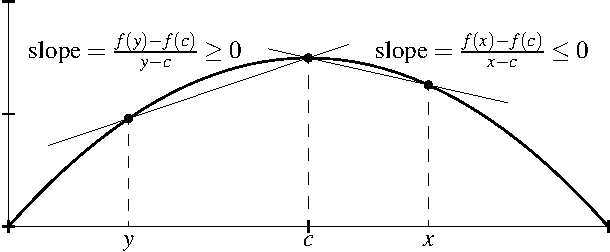
\includegraphics{figures/critpt}
\caption{Slopes of secants at a relative maximum.\label{fig:critpt}}
\end{myfigureht}

As $a < c < b$, there exist
sequences $\{ x_n\}$ and $\{ y_n \}$, such
that $x_n > c$, and
$y_n < c$ for all $n \in \N$, and such that
 $\lim\, x_n = \lim\, y_n = c$.
Since $f$
is differentiable at $c$ we know 
\begin{equation*}
0 \geq \lim_{n\to\infty} \frac{f(x_n)-f(c)}{x_n-c} 
=
f'(c)
=
\lim_{n\to\infty} \frac{f(y_n)-f(c)}{y_n-c} \geq 0.  \qedhere
\end{equation*}
\end{proof}

For a differentiable function, a point where 
$f'(c) = 0$ is called a \emph{\myindex{critical point}}.  When $f$ is not
differentiable at some points,
it is common to also say $c$ is a critical point
if $f'(c)$ does not exist.
The theorem says that a relative minimum or maximum at an interior point
of an interval must be a critical point.
As you remember from calculus, finding minima and maxima of a function can
be done by finding all the critical points together with the endpoints of
the interval and simply checking at which of these points
is the function biggest or smallest.

\subsection{Rolle's theorem}

Suppose a function has the same value at both endpoints of an interval.
Intuitively it ought to attain a minimum or a maximum in the interior of the
interval,
then at such a minimum or a maximum, the derivative should be zero.
See \figureref{rollefig} for the geometric idea.  This is the content of the
so-called Rolle's theorem%
\footnote{Named after the French mathematician
\href{https://en.wikipedia.org/wiki/Michel_Rolle}{Michel Rolle}
(1652--1719).}.

\begin{myfigureht}
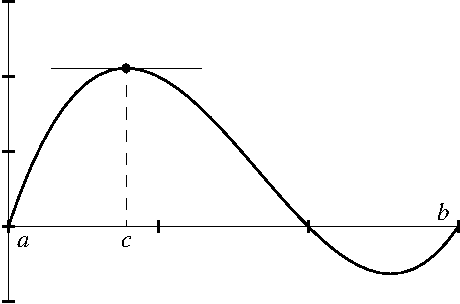
\includegraphics{figures/rollefig}
\caption{Point where tangent line is horizontal, that is $f'(c) =
0$.\label{rollefig}}
\end{myfigureht}

\begin{thm}[Rolle] \label{thm:rolle}
\index{Rolle's theorem}
Let $f \colon [a,b] \to \R$ be continuous function
differentiable on $(a,b)$ such that $f(a) = f(b)$.
Then there exists a $c \in (a,b)$ such that $f'(c) = 0$.
\end{thm}

\begin{proof}
As $f$ is continuous on $[a,b]$ it attains an absolute minimum and an
absolute 
maximum in $[a,b]$.  We wish to apply \lemmaref{relminmax:lemma} and
so we need a minimum or maximum at some $c \in (a,b)$.
Write $K := f(a) = f(b)$.
If there exists an $x$ such that $f(x) > K$, then the absolute
maximum is bigger than $K$ and hence occurs at $c \in (a,b)$, and
therefore we get $f'(c) = 0$.  On the other hand if there exists an $x$
such that $f(x) < K$, then the absolute minimum occurs at some
$c \in (a,b)$ and we have that $f'(c) = 0$.  If there is no $x$ such that
$f(x) > K$ or
$f(x) < K$, then we have that $f(x) = K$ for all $x$ and then
$f'(x) = 0$ for all $x \in [a,b]$, so any $c \in (a,b)$ works.
\end{proof}

It is absolutely necessary for the derivative to exist for all $x
\in (a,b)$.  For example take the function $f(x) = \abs{x}$ on $[-1,1]$.
Clearly $f(-1) = f(1)$, but there is no point where $f'(c) = 0$.

\subsection{Mean value theorem}

We extend \hyperref[thm:rolle]{Rolle's theorem}
to functions that attain different
values at the endpoints.

\begin{thm}[Mean value theorem] \label{thm:mvt}
\index{mean value theorem}
Let $f \colon [a,b] \to \R$ be a continuous function
differentiable on $(a,b)$.  Then there exists a point $c \in (a,b)$
such that
\begin{equation*}
f(b)-f(a) = f'(c)(b-a) .
\end{equation*}
\end{thm}

For a geometric interpretation of the mean value theorem, see
\figureref{mvtfig}.  The idea is that the value $\frac{f(b)-f(a)}{b-a}$
is the slope of the line between the points $\bigl(a,f(a)\bigr)$
and $\bigl(b,f(b)\bigr)$.
Then $c$ is the point such that $f'(c) = \frac{f(b)-f(a)}{b-a}$, that 
is, the tangent line at the point $\bigl(c,f(c)\bigr)$ has the same slope as the
line between $\bigl(a,f(a)\bigr)$ and $\bigl(b,f(b)\bigr)$.
The theorem follows from \hyperref[thm:rolle]{Rolle's theorem},
by subtracting from $f$ the affine linear function with the derivative
$\frac{f(b)-f(a)}{b-a}$ with the same values at $a$ and $b$ as $f$.
That is, we subtract the function whose graph is the straight line
$\bigl(a,f(a)\bigr)$ and $\bigl(b,f(b)\bigr)$.
Then we are looking for a point where this new
function has derivative zero.

\begin{myfigureht}
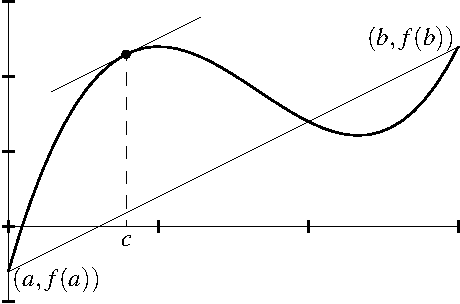
\includegraphics{figures/mvtfig}
\caption{Graphical interpretation of the mean value theorem.\label{mvtfig}}
\end{myfigureht}


\begin{proof}
Define the
function $g \colon [a,b] \to \R$ by
\begin{equation*}
g(x) := f(x)-f(b)-\frac{f(b)-f(a)}{b-a}(x-b) .
\end{equation*}
The function $g$ is differentiable on $(a,b)$,
continuous on $[a,b]$, such that $g(a) = 0$ and $g(b) = 0$.  Thus there exists
a
$c \in (a,b)$ such that $g'(c) = 0$.
\begin{equation*}
0 = g'(c) = f'(c)-\frac{f(b)-f(a)}{b-a}
\end{equation*}
Or in other words
$f'(c)(b-a) = f(b)-f(a)$.
\end{proof}

The proof generalizes.  By considering
$g(x) :=
f(x)-f(b)-\frac{f(b)-f(a)}{\varphi(b)-\varphi(a)}\bigl(\varphi(x)-\varphi(b)\bigr)$
one can prove the following version.  We leave the proof as an exercise.

\begin{thm}[Cauchy's mean value theorem] \label{thm:cauchymvt}
\index{Cauchy's mean value theorem}
Let $f \colon [a,b] \to \R$ and $\varphi \colon [a,b] \to \R$ be continuous
functions
differentiable on $(a,b)$.  Then there exists a point $c \in (a,b)$
such that
\begin{equation*}
\bigl(f(b)-f(a)\bigr)\varphi'(c) = f'(c)\bigl(\varphi(b)-\varphi(a)\bigr) .
\end{equation*}
\end{thm}

The mean value theorem has the distinction of being one of the few theorems
commonly cited
in court.  That is, when police measure the speed of cars by aircraft, or
via cameras reading license plates, they 
measure the time the car takes to go between two points.
The mean value theorem then
says that the car must have somewhere attained the speed you get by dividing the
difference in distance by the difference in time.



\subsection{Applications}

We now solve our very first differential equation.

\begin{prop} \label{prop:derzeroconst}
Let $I$ be an interval and
let $f \colon I \to \R$ be a differentiable function such that $f'(x) = 0$
for all $x \in I$.
Then $f$ is constant.
\end{prop}

\begin{proof}
Take arbitrary $x,y \in I$ with $x < y$.
Then $f$ restricted to $[x,y]$ satisfies the hypotheses
of the \hyperref[thm:mvt]{mean value theorem}.
Therefore there is a $c \in (x,y)$ such that
\begin{equation*}
f(y)-f(x) = f'(c)(y-x).
\end{equation*}
as $f'(c) = 0$, we have $f(y) = f(x)$.  Therefore,
the function is constant.
\end{proof}

Now that we know what it means for the function to stay constant, let us look
at increasing and decreasing functions.
We say $f \colon I \to \R$ is \emph{\myindex{increasing}}
(resp.\  \emph{\myindex{strictly increasing}}) if
$x < y$ implies $f(x) \leq f(y)$ (resp.\ $f(x) < f(y)$).
We define
\emph{\myindex{decreasing}} and
\emph{\myindex{strictly decreasing}} in the same way by switching the
inequalities for $f$.

\begin{prop} \label{incdecdiffprop}
Let $I$ be an interval and
let $f \colon I \to \R$ be a differentiable function.
%\begin{enumerate}[(i),itemsep=0.5\itemsep,parsep=0.5\parsep,topsep=0.5\topsep,partopsep=0.5\partopsep]
\begin{enumerate}[(i)]
\item $f$ is increasing if and only if $f'(x) \geq 0$ for all $x \in I$.
\item $f$ is decreasing if and only if $f'(x) \leq 0$ for all $x \in I$.
\end{enumerate}
\end{prop}

\begin{proof}
Let us prove the first item.  Suppose $f$ is increasing, then
for all $x,c \in I$ with $x \neq c$ we have
\begin{equation*}
\frac{f(x)-f(c)}{x-c} \geq 0 .
\end{equation*}
Taking a limit as $x$ goes to $c$ we see that $f'(c) \geq 0$.

For the other direction, suppose $f'(x) \geq 0$ for all $x \in I$.
Take any $x, y \in I$ where $x < y$.  By the \hyperref[thm:mvt]{mean value theorem}
there is some $c \in
(x,y)$ such that
\begin{equation*}
f(y)-f(x) = f'(c)(y-x) .
\end{equation*}
As $f'(c) \geq 0$, and $y-x > 0$, then $f(y) - f(x) \geq 0$ or $f(x) \leq
f(y)$ and so
$f$ is increasing.

We leave the decreasing part to the reader as exercise.
\end{proof}

A similar but weaker statement is true for strictly increasing and
decreasing functions.

\begin{prop} \label{incdecdiffstrictprop}
Let $I$ be an interval and
let $f \colon I \to \R$ be a differentiable function.
\begin{enumerate}[(i)]
\item
\label{incdecdiffstrictprop:i}
If $f'(x) > 0$ for all $x \in I$, then
$f$ is strictly increasing.
\item
\label{incdecdiffstrictprop:ii}
If $f'(x) < 0$ for all $x \in I$,
then $f$ is strictly decreasing.
\end{enumerate}
\end{prop}

The proof of
\ref{incdecdiffstrictprop:i}
is left as an exercise.
Then \ref{incdecdiffstrictprop:ii}
follows from 
\ref{incdecdiffstrictprop:i} by considering $-f$
instead.

The converse of this proposition is not true.  For example,
$f(x) := x^3$ is a strictly increasing function, but $f'(0) = 0$.

\medskip

Another application of the \hyperref[thm:mvt]{mean value theorem} is the following result about
location of extrema, sometimes called the \emph{\myindex{first derivative
test}}.  The theorem is stated for an absolute minimum and
maximum. To apply it to find relative minima
and maxima, restrict $f$ to an interval $(c-\delta,c+\delta)$.

\begin{prop} \label{firstderminmaxtest}
Let $f \colon (a,b) \to \R$ be continuous.  Let $c \in (a,b)$
and suppose
$f$ is differentiable on $(a,c)$ and $(c,b)$.
\begin{enumerate}[(i)]
\item If $f'(x) \leq 0$ for $x \in (a,c)$ and
 $f'(x) \geq 0$ for $x \in (c,b)$, then $f$ has an absolute minimum 
at $c$.
\item If $f'(x) \geq 0$ for $x \in (a,c)$ and
 $f'(x) \leq 0$ for $x \in (c,b)$, then $f$ has an absolute maximum
at $c$.
\end{enumerate}
\end{prop}

\begin{proof}
We prove the first item leaving the second to the reader.
Take $x \in (a,c)$
and $\{ y_n\}$ a sequence such that $x < y_n < c$ and $\lim\, y_n = c$.
By the preceding proposition,
$f$ is decreasing on $(a,c)$ so $f(x) \geq f(y_n)$.
As $f$ is
continuous at $c$, we take the limit to get
$f(x) \geq f(c)$ for all $x \in (a,c)$.

Similarly take $x \in (c,b)$
and $\{ y_n\}$ a sequence such that $c < y_n < x$ and $\lim\, y_n = c$.
The function is increasing on $(c,b)$ so $f(x) \geq f(y_n)$.
By continuity of $f$ we get
$f(x) \geq f(c)$ for all $x \in (c,b)$.  Thus $f(x) \geq f(c)$ for all
$x \in (a,b)$.
\end{proof}

The converse of the proposition does not hold.  See
\exampleref{baddifffunc:example} below.

\subsection{Continuity of derivatives and the intermediate value theorem}

Derivatives of functions satisfy an
intermediate value property.

\begin{thm}[Darboux] \label{thm:darboux} \index{Darboux's theorem}
Let $f \colon [a,b] \to \R$ be differentiable.  Suppose $y \in \R$ is such
that $f'(a) < y < f'(b)$ or
$f'(a) > y > f'(b)$.  Then there exists a $c \in (a,b)$ such that $f'(c) =
y$.
\end{thm}

The proof follows by subtracting $f$ and a linear function with derivative
$y$.  The new function $g$ reduces the problem
to the case $y=0$, where $g'(a) > 0 > g'(b)$.  That is, $g$ is increasing at $a$ and
decreasing at $b$, so it must attain a maximum inside $(a,b)$,
where the derivative is zero.  See \figureref{darbouxthmfig}.

\begin{myfigureht}
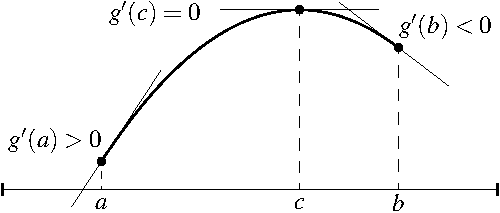
\includegraphics{figures/darbouxthmfig}
\caption{Idea of the proof of Darboux theorem.\label{darbouxthmfig}}
\end{myfigureht}

\begin{proof}
Suppose 
$f'(a) < y < f'(b)$.
Define
\begin{equation*}
g(x) := yx - f(x) .
\end{equation*}
The function $g$ is continuous on $[a,b]$, and so $g$ attains a maximum at some $c \in
[a,b]$.

The function $g$ is also differentiable on $[a,b]$.
Compute $g'(x) = y-f'(x)$.  Thus $g'(a) > 0$.  As the derivative is
the limit of difference quotients and is positive, there must be some
difference quotient that is positive.  That is, there must exist
an $x > a$ such that
\begin{equation*}
\frac{g(x)-g(a)}{x-a} > 0 ,
\end{equation*}
or $g(x) > g(a)$.  Thus $g$
cannot possibly have a maximum at $a$.  Similarly as $g'(b) < 0$,
we find an $x < b$ (a different $x$) such that
$\frac{g(x)-g(b)}{x-b} < 0$ or that $g(x) > g(b)$, thus
$g$ cannot possibly have a maximum at $b$.
Therefore $c \in (a,b)$
and \hyperref[thm:rolle]{Rolle's theorem} applies: As $g$ attains a maximum
at $c$ we find $g'(c) = 0$
and $f'(c) = y$.

Similarly if $f'(a) > y > f'(b)$, consider $g(x) := f(x)- yx$.
\end{proof}

We have seen already that
there exist discontinuous functions that have the
intermediate value property.  While it is hard to imagine at first, there
also
exist functions that are differentiable everywhere and the derivative is not
continuous.

\begin{example} \label{baddifffunc:example}
Let $f \colon \R \to \R$ be the function defined by
\begin{equation*}
f(x) :=
\begin{cases}
{\bigl( x \sin(\nicefrac{1}{x}) \bigr)}^2 & \text{ if $x \not= 0$,} \\
0 & \text{ if $x = 0$.}
\end{cases}
\end{equation*}
We claim that $f$ is differentiable everywhere, but
$f' \colon \R \to \R$ is not continuous at
the origin.  Furthermore, $f$ has a minimum at 0, but the derivative
changes sign infinitely often near the origin.
See \figureref{fig:nonc1diff}.
\begin{myfigureht}
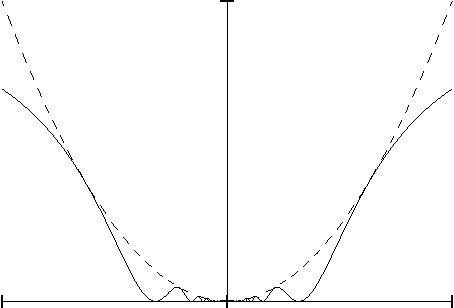
\includegraphics{figures/nonc1difffig}
\qquad
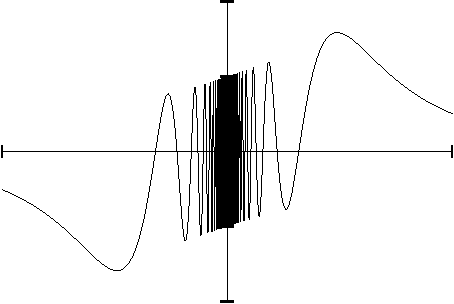
\includegraphics{figures/nonc1diffderfig}
\caption{A function with a discontinuous derivative. The function $f$ is on the left
and $f'$ is on the right.  Notice that $f(x) \leq x^2$ on the left graph.\label{fig:nonc1diff}}
\end{myfigureht}

Proof: It is immediate from the definition that $f$ has an absolute
minimum at 0: we know $f(x) \geq 0$ for all $x$ and $f(0) = 0$.

The function $f$ is differentiable for $x\not=0$,
and
the derivative 
is $2 \sin (\nicefrac{1}{x}) \bigl( x \sin (\nicefrac{1}{x}) -
\cos(\nicefrac{1}{x}) \bigr)$.
As an exercise show that for $x_n = \frac{4}{(8n+1)\pi}$
we have
$\lim\, f'(x_n) = -1$, and for
$y_n = \frac{4}{(8n+3)\pi}$  we have
$\lim\, f'(y_n) = 1$.  Hence if $f'$ exists at $0$,
then it cannot be continuous.

Let us show that $f'$ exists at 0.  We claim that the derivative is zero.
In other words $\abs{\frac{f(x)-f(0)}{x-0} - 0}$ goes to zero
as $x$ goes to zero.  For $x \not= 0$ we have
\begin{equation*}
\abs{\frac{f(x)-f(0)}{x-0} - 0}
=
\abs{\frac{x^2 \sin^2(\nicefrac{1}{x})}{x}}
=
\abs{x \sin^2(\nicefrac{1}{x})}
\leq
\abs{x} .
\end{equation*}
And, of course, as $x$ tends to zero, then $\abs{x}$ tends to zero and hence
$\abs{\frac{f(x)-f(0)}{x-0} - 0}$ goes to zero.  Therefore, $f$
is differentiable at 0 and the derivative at 0 is 0.
A key point in the above calculation is that 
is that $\abs{f(x)} \leq x^2$,
see also Exercises \ref{exercise:bndmuldiff} and
\ref{exercise:diffsqueeze}.
\end{example}

It is sometimes useful to assume the derivative of a differentiable
function is continuous.  If $f \colon I \to \R$ is differentiable and
the derivative $f'$ is continuous on $I$, then we say $f$ is
\emph{\myindex{continuously
differentiable}}\index{differentiable!continuously}.  It is common to
write $C^1(I)$ for the set of continuously differentiable functions on $I$.

\subsection{Exercises}

\begin{exercise}
Finish the proof of \propref{incdecdiffprop}.
\end{exercise}

\begin{exercise}
Finish the proof of \propref{firstderminmaxtest}.
\end{exercise}

\begin{exercise} \label{exercise:boundeddermeanslip}
Suppose $f \colon \R \to \R$ is a differentiable
function such that $f'$ is a bounded function.  Prove
$f$ is a Lipschitz continuous function.
\end{exercise}

\begin{exercise}
Suppose $f \colon [a,b] \to \R$ is differentiable and $c \in [a,b]$.
Then show there exists a sequence $\{ x_n \}$ converging to $c$, $x_n
\not= c$ for all $n$, such that
\begin{equation*}
f'(c) = \lim_{n\to \infty} f'(x_n).
\end{equation*}
Do note this does \emph{not} imply that $f'$ is continuous (why?).
\end{exercise}

\begin{exercise}
Suppose $f \colon \R \to \R$ is a function such that
$\abs{f(x)-f(y)} \leq \abs{x-y}^2$ for all $x$ and $y$.  Show that
$f(x) = C$ for some constant $C$.  Hint: Show that $f$ is differentiable
at all points and compute the derivative.
\end{exercise}

\begin{exercise} \label{exercise:posderincr}
Finish the proof of \propref{incdecdiffstrictprop}.  That is,
suppose $I$ is an interval and
$f \colon I \to \R$ is a differentiable function.
If $f'(x) > 0$ for all $x \in I$, show that $f$ is strictly increasing.
\end{exercise}

\begin{exercise}
Suppose $f \colon (a,b) \to \R$ is a differentiable function
such that
$f'(x) \not= 0$ for all $x \in (a,b)$.  Suppose there
exists
a point $c \in (a,b)$ such that $f'(c) > 0$.
Prove $f'(x) > 0$ for all $x \in (a,b)$.
\end{exercise}

\begin{exercise} \label{exercise:samediffconst}
Suppose $f \colon (a,b) \to \R$ and $g \colon (a,b) \to \R$ are
differentiable functions such that $f'(x) = g'(x)$ for all $x \in (a,b)$,
then show that there exists a constant $C$ such that $f(x) = g(x) + C$.
\end{exercise}

\begin{exercise}
Prove the following version of \myindex{L'H\^opital's rule}\index{L'Hospital's rule}.
Suppose 
$f \colon (a,b) \to \R$ and $g \colon (a,b) \to \R$ are differentiable
functions.  Suppose that at $c \in (a,b)$, $f(c) = 0$, $g(c)=0$,
$g'(x) \not= 0$ when $x \not= c$, and
that the limit of $\nicefrac{f'(x)}{g'(x)}$ as $x$ goes to $c$ exists.  Show that
\begin{equation*}
\lim_{x \to c} \frac{f(x)}{g(x)} = 
\lim_{x \to c} \frac{f'(x)}{g'(x)} .
\end{equation*}
Compare to \exerciseref{exercise:simpleLHopital}.
\end{exercise}

\begin{exercise}
Let $f \colon (a,b) \to \R$ be an unbounded differentiable function.  Show
$f' \colon (a,b) \to \R$ is unbounded.
\end{exercise}

\begin{exercise}
Prove the theorem Rolle actually proved in 1691:
\emph{If $f$ is a polynomial,
$f'(a) = f'(b) = 0$ for some $a < b$,
and there is no $c \in (a,b)$ such that $f'(c) = 0$,
then there is at most one root of $f$ in $(a,b)$,
that is at most one $x \in (a,b)$ such that $f(x) = 0$.}
In other words, between any two consecutive roots of $f'$ is at most one
root of $f$.
Hint: Suppose there are two roots and see what happens.
\end{exercise}

\begin{exercise}
Suppose $a,b \in \R$ and $f \colon \R \to \R$ is differentiable,
$f'(x) = a$ for all $x$, and $f(0) = b$.  Find $f$ and prove that 
it is the unique differentiable function with this property.
\end{exercise}

\begin{exercise} \label{exercise:extendboundedder}
Suppose $f \colon (0,1) \to \R$ is differentiable and $f'$
is bounded.
\begin{enumerate}[a)]
\item
Show that there exists a continuous function $g \colon [0,1) \to \R$
such that $f(x) = g(x)$ for all $x \not= 0$.  Hint: \propref{context:prop} and
\exerciseref{exercise:boundeddermeanslip}.
\item
Find an example where the $g$ is not differentiable at $x=0$.
Hint: Consider something based on $\sin(\ln x)$,
and assume you know basic properties of
$\sin$ and $\ln$ from calculus.
\end{enumerate}
\end{exercise}

\begin{exercise}
Suppose $f \colon (a,b) \to \R$ is differentiable everywhere except at $c \in
(a,b)$ and $\lim_{x \to c} f'(x) = L$.  Show that $f$ is differentiable at
$c$ and $f'(c) = L$.
\end{exercise}

\begin{exercise}
Prove \thmref{thm:cauchymvt}.
\end{exercise}

%%%%%%%%%%%%%%%%%%%%%%%%%%%%%%%%%%%%%%%%%%%%%%%%%%%%%%%%%%%%%%%%%%%%%%%%%%%%%%

\sectionnewpage
\section{Taylor's theorem}
\label{sec:taylor}

\sectionnotes{less than a lecture (optional section)}

\subsection{Derivatives of higher orders}

When $f \colon I \to \R$ is differentiable, we obtain a function
$f' \colon I \to \R$.  The function
$f'$ is called the \emph{\myindex{first derivative}} of $f$.
If $f'$ is differentiable, we denote by
$f'' \colon I \to \R$ the derivative of $f'$.  The function $f''$
is called the \emph{\myindex{second derivative}} of $f$.
\glsadd{not:secondthirdfourthder}
We similarly obtain
$f'''$, $f''''$, and so on.
With a larger number of derivatives
the notation would get out of hand; we denote
by $f^{(n)}$ the
\glsadd{not:nthder}
\emph{$n$th derivative}\index{nth derivative@$n$th derivative} of $f$.

When $f$ possesses $n$ derivatives, we say $f$ is
\emph{$n$ times differentiable}\index{n times differentiable@$n$ times
differentiable}\index{differentiable!n times@$n$ times}.

\subsection{Taylor's theorem}

Taylor's theorem%
\footnote{Named for the English mathematician
\href{http://en.wikipedia.org/wiki/Brook_Taylor}{Brook Taylor}
(1685--1731).
It was first found by
the Scottish mathematician
\href{http://en.wikipedia.org/wiki/James_Gregory_(mathematician)}{James Gregory}
(1638--1675).  The statement we give
was proved by
\href{http://en.wikipedia.org/wiki/Lagrange}{Joseph-Louis Lagrange}
(1736--1813)}
is a generalization of the \hyperref[thm:mvt]{mean value theorem}.
Mean value theorem says that up to a small error $f(x)$ for $x$ near $x_0$ can be
approximated by $f(x_0)$, that is
\begin{equation*}
f(x) = f(x_0) + f'(c)(x-x_0),
\end{equation*}
where the ``error'' is measured in terms of the first derivative
at some point $c$ between $x$ and $x_0$.
Taylor's theorem generalizes this result to higher derivatives.
It tells us that up to a small error, any $n$
times differentiable function can be approximated at a point $x_0$
by a polynomial.  The
error of this approximation behaves like ${(x-x_0)}^{n}$ near the point $x_0$.
To see why this is a good approximation notice that for a big $n$, 
${(x-x_0)}^n$ is very small in a small interval around $x_0$.

\begin{defn}
For an $n$ times differentiable function $f$ defined near a point $x_0 \in \R$, define the
$n$th order \emph{\myindex{Taylor polynomial}}%
\index{nth order Taylor polynomial@$n$th order Taylor polynomial}
for $f$ at $x_0$ as
\begin{equation*}
\begin{split}
P_n^{x_0}(x)
& :=
\sum_{k=0}^n
\frac{f^{(k)}(x_0)}{k!}{(x-x_0)}^k
\\
& =
f(x_0)
+ f'(x_0)(x-x_0)
+ \frac{f''(x_0)}{2}{(x-x_0)}^2
+ \frac{f^{(3)}(x_0)}{6}{(x-x_0)}^3
+ \cdots
+ \frac{f^{(n)}(x_0)}{n!}{(x-x_0)}^n .
\end{split}
\end{equation*}
\end{defn}

See \figureref{fig:taylorsin} for
the odd degree Taylor polynomials for the sin function at $x_0=0$.
The even degree terms are all zero, as even derivatives 
of sine are again a sine, which are zero at the origin.
\begin{myfigureht}
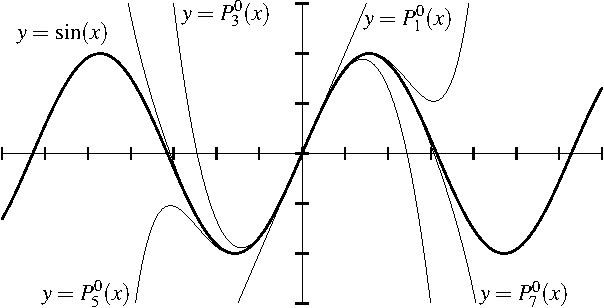
\includegraphics{figures/taylorsin}
\caption{The odd degree Taylor polynomials for the sine
function.\label{fig:taylorsin}}
\end{myfigureht}

Taylor's theorem says a function behaves like its $n$th
Taylor polynomial.  The 
\hyperref[thm:mvt]{mean value theorem} is really Taylor's theorem
for the first derivative.

\begin{thm}[Taylor]\index{Taylor's theorem} \label{thm:taylor}
Suppose $f \colon [a,b] \to \R$ is a function with $n$ continuous
derivatives on $[a,b]$ and such that $f^{(n+1)}$ exists on $(a,b)$.
Given distinct points $x_0$ and $x$ in $[a,b]$,
we can find a point $c$ between $x_0$
and $x$ such that
\begin{equation*}
f(x)=P_{n}^{x_0}(x)+\frac{f^{(n+1)}(c)}{(n+1)!}{(x-x_0)}^{n+1} .
\end{equation*}
\end{thm}

The term $R_n^{x_0}(x):=\frac{f^{(n+1)}(c)}{(n+1)!}{(x-x_0)}^{n+1}$ is called the
\emph{remainder term}\index{remainder term in Taylor's formula}.  This
form 
of the remainder term is called the
\emph{\myindex{Lagrange form}} of the remainder.  There are other ways
to write the remainder term, but we skip those.  Note that $c$ depends on
both $x$ and $x_0$.

\begin{proof}
Find a number $M_{x,x_0}$ (depending on $x$ and $x_0$) solving the equation
\begin{equation*}
f(x)=P_{n}^{x_0}(x)+M_{x,x_0}{(x-x_0)}^{n+1} .
\end{equation*}
Define a function $g(s)$ by
\begin{equation*}
g(s) := f(s)-P_n^{x_0}(s)-M_{x,x_0}{(s-x_0)}^{n+1} .
\end{equation*}
We compute
the $k$th derivative at $x_0$ of the Taylor polynomial
${(P_n^{x_0})}^{(k)}(x_0) = f^{(k)}(x_0)$ for
$k=0,1,2,\ldots,n$ (the zeroth derivative of a function is the function
itself).  Therefore,
\begin{equation*}
g(x_0) = g'(x_0) = g''(x_0) = \cdots = g^{(n)}(x_0) = 0 .
\end{equation*}
In particular $g(x_0) = 0$.
On the other hand $g(x) = 0$.  By the
\hyperref[thm:mvt]{mean value theorem}
there exists an $x_1$ between $x_0$ and $x$ such that $g'(x_1) = 0$.
Applying the \hyperref[thm:mvt]{mean value theorem}
to $g'$ we obtain that there exists
$x_2$ between $x_0$ and $x_1$ (and therefore between $x_0$ and $x$)
such that $g''(x_2) = 0$.  We repeat the
argument $n+1$ times to obtain a number $x_{n+1}$ between $x_0$ and $x_n$
(and therefore between $x_0$ and $x$) such that $g^{(n+1)}(x_{n+1}) = 0$.

Let $c:=x_{n+1}$.
We compute the $(n+1)$th derivative of $g$ to find
\begin{equation*}
g^{(n+1)}(s) = f^{(n+1)}(s)-(n+1)!\,M_{x,x_0} .
\end{equation*}
Plugging in $c$ for $s$ we obtain $M_{x,x_0} = \frac{f^{(n+1)}(c)}{(n+1)!}$, and
we are done.
\end{proof}

In the proof we have computed 
${(P_n^{x_0})}^{(k)}(x_0) = f^{(k)}(x_0)$ for $k=0,1,2,\ldots,n$.
Therefore the Taylor polynomial has the same derivatives as $f$ at $x_0$
up to the $n$th derivative.  That is why the Taylor polynomial is
a good approximation to $f$.
Notice that in \figureref{fig:taylorsin} the Taylor polynomials are
reasonably good approximations to the sine near $x=0$.

We do not necessarily get good approximations
by the Taylor polynomial everywhere.
For example, if we start expanding the function $f(x) =
\frac{x}{1-x}$ around 0, we get the graphs in
\figureref{fig:taylorgeom}.  The dotted lines are the first, second, and
third degree approximations.  The dashed line is
the 20th degree polynomial, and yet the approximation only seems to get
better with the degree for $x > -1$, and for smaller $x$, it in fact gets worse.
The polynomials
are the partial sums of the geometric series $\sum_{n=1}^\infty x^n$,
and the series only converges on $(-1,1)$.
See the discussion of power series
\sectionref{sec:moreonseries}.

\begin{myfigureht}
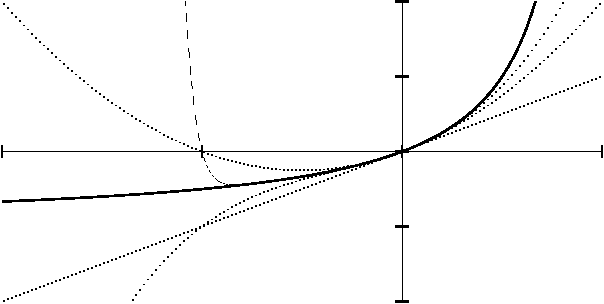
\includegraphics{figures/taylorgeom}
\caption{The function $\frac{x}{1-x}$, and the Taylor polynomials
$P_1^0$, $P_2^0$, $P_3^0$ (all dotted), and the polynomial $P_{20}^0$
(dashed).\label{fig:taylorgeom}}
\end{myfigureht}

If $f$ is \emph{\myindex{infinitely
differentiable}}\index{differentiable!infinitely},
that is, if $f$ can be
differentiated any number of times, then 
we define the \emph{\myindex{Taylor series}}:
\begin{equation*}
%T^{x_0}(x)
%:=
\sum_{k=0}^\infty
\frac{f^{(k)}(x_0)}{k!}{(x-x_0)}^k .
\end{equation*}
There is no guarantee that this series converges for any
$x \not= x_0$.  And even where it does converge, there is no guarantee
that it converges to the function $f$.  Functions for which
the Taylor series converges to the function at least in an interval
around every point are called
\emph{\myindex{analytic functions}}\index{analytic function}.
Most functions one tends to see in practice are in fact analytic.
See \exerciseref{exercise:nonanalytic}, for an example of a non-analytic
function.

\medskip

The definition of derivative says that
a function is
differentiable if it
is locally approximated by a line.
%, that is the definition of the derivative.
Similarly we mention in passing that there exists a converse to Taylor's
theorem,
which we will neither state nor prove,
saying that if a function is
locally approximated in a certain way by a polynomial of degree $d$, then it
has $d$ derivatives.

\medskip

Taylor's theorem gives us a quick proof of a version of
the second derivative test.
By a \emph{\myindex{strict relative minimum}}\index{minimum!strict relative}
of $f$ at $c$,
we mean that there exists a $\delta > 0$ such that $f(x) > f(c)$ for
all $x \in (c-\delta,c+\delta)$ where $x\not=c$.
A \emph{\myindex{strict relative maximum}}\index{minimum!strict relative}
is defined similarly.
Continuity of the second derivative is not needed, but the proof is more
difficult and is left as an exercise.  The proof also generalizes
immediately into the $n$th derivative test, which is also left as
an exercise.

\begin{prop}[Second derivative test]\index{second derivative test}
Suppose $f \colon (a,b) \to \R$ is twice continuously differentiable,
$x_0 \in (a,b)$, $f'(x_0) = 0$ and $f''(x_0) > 0$.  Then $f$ has a strict relative
minimum at $x_0$.
\end{prop}

\begin{proof}
As $f''$ is continuous, there exists a $\delta > 0$
such that $f''(c) > 0$ for all $c \in (x_0-\delta,x_0+\delta)$,
see \exerciseref{exercise:positivecontneigh}.
Take $x \in (x_0-\delta,x_0+\delta)$, $x \not= x_0$.
Taylor's theorem says that for some $c$ between $x_0$ and $x$,
\begin{equation*}
f(x) 
=
f(x_0) + f'(x_0) (x-x_0) +
\frac{f''(c)}{2}{(x-x_0)}^{2} 
=
f(x_0) + \frac{f''(c)}{2}{(x-x_0)}^{2}  .
\end{equation*}
As $f''(c) > 0$, and ${(x-x_0)}^2 > 0$, then $f(x) > f(x_0)$.
\end{proof}

\subsection{Exercises}

\begin{exercise}
Compute the $n$th Taylor Polynomial at $0$ for the exponential function.
\end{exercise}

\begin{exercise}
Suppose $p$ is a polynomial of degree $d$.  Given any $x_0 \in \R$,
show that
the $(d+1)$th Taylor polynomial for $p$ at $x_0$ is equal to $p$.
\end{exercise}

\begin{exercise}
Let $f(x) := \abs{x}^3$.  Compute $f'(x)$ and $f''(x)$ for all $x$,
but show that $f^{(3)}(0)$ does not exist.
\end{exercise}

\begin{exercise}
Suppose $f \colon \R \to \R$ has $n$ continuous derivatives.  Show
that for any $x_0 \in \R$,
there exist polynomials $P$ and $Q$ of degree $n$ and 
an $\epsilon > 0$ such that $P(x) \leq f(x) \leq Q(x)$ for all $x \in
[x_0-\epsilon,x_0+\epsilon]$  and
$Q(x)-P(x) = \lambda {(x-x_0)}^n$ for some $\lambda \geq 0$.
\end{exercise}

\begin{exercise}
If $f \colon [a,b] \to \R$ has $n+1$ continuous derivatives
and $x_0 \in [a,b]$,
prove
$\lim\limits_{x\to x_0} \frac{R_n^{x_0}(x)}{{(x-x_0)}^n} = 0$.
\end{exercise}

\begin{exercise}
Suppose $f \colon [a,b] \to \R$ has $n+1$ continuous derivatives
and $x_0 \in (a,b)$.
Prove: $f^{(k)}(x_0) = 0$ for all $k = 0, 1, 2, \ldots, n$
if and only if $g(x) := \frac{f(x)}{{(x-x_0)}^{n+1}}$ is continuous at $x_0$.
\end{exercise}

\begin{exercise}
Suppose $a,b,c \in \R$ and $f \colon \R \to \R$ is differentiable,
$f''(x) = a$ for all $x$, $f'(0) = b$, and $f(0) = c$.  Find $f$ and prove that 
it is the unique differentiable function with this property.
\end{exercise}

\begin{exercise}[Challenging]
Show that a simple converse to Taylor's theorem does not hold.
Find a function $f \colon \R \to \R$ with no second derivative at $x=0$ such that
$\abs{f(x)} \leq \abs{x^3}$, that is, $f$ goes to zero at 0 faster than $x^3$, and
while $f'(0)$ exists, $f''(0)$ does not.
\end{exercise}

\begin{exercise} \label{exercise:extendboundedder2}
Suppose $f \colon (0,1) \to \R$ is differentiable and $f''$
is bounded.
\begin{enumerate}[a)]
\item
Show that there exists a once differentiable function $g \colon [0,1) \to \R$
such that $f(x) = g(x)$ for all $x \not= 0$.  Hint: 
See
\exerciseref{exercise:extendboundedder}.
\item
Find an example where the $g$ is not twice differentiable at $x=0$.
\end{enumerate}
\end{exercise}

\begin{exercise}
Prove the
\emph{$n$th derivative test}\index{nth derivative test@$n$th derivative test}.
Suppose $n \in \N$,
$x_0 \in (a,b)$, and $f \colon (a,b) \to \R$ is $n$ times continuously
differentiable, with $f^{(k)}(x_0) = 0$ for $k=1,2,\ldots,n-1$, and
$f^{(n)}(x_0)
\not= 0$.
Prove:
\begin{enumerate}[a)]
\item
If $n$ is odd then $f$ has neither a relative minimum,
nor a maximum at $x_0$.
\item
If $n$ is even then $f$ has a strict relative minimum at $x_0$ if
$f^{(n)}(x_0) > 0$
and a strict relative maximum at $x_0$ if $f^{(n)}(x_0) < 0$.
\end{enumerate}
\end{exercise}

\begin{exercise}
Prove the more general version of the second derivative test.
Suppose $f \colon (a,b) \to \R$ is differentiable and $x_0 \in (a,b)$
is such that $f''(x_0)$ exists and $f''(x_0) > 0$.
Prove that $f$ has a strict relative
minimum at $x_0$.  Hint: Consider the limit definition of $f''(x_0)$.
\end{exercise}

%%%%%%%%%%%%%%%%%%%%%%%%%%%%%%%%%%%%%%%%%%%%%%%%%%%%%%%%%%%%%%%%%%%%%%%%%%%%%%

\sectionnewpage
\section{Inverse function theorem}
\label{sec:ift}

\sectionnotes{less than 1 lecture (optional section, needed for
\sectionref{sec:logandexp}, requires 
\sectionref{sec:monotonefunc})}

\subsection{Inverse function theorem}

Let us start with a simple example.  Consider a function $f(x) := a x$ for a
number $a \not= 0$.  Then $f \colon \R \to \R$ is bijective, and the inverse
is $f^{-1}(y) = \frac{1}{a} y$.  In particular, $f'(x) = a$ and 
$(f^{-1})'(y) = \frac{1}{a}$.  As differentiable functions are
``infinitesimally like'' linear functions, then we expect the same
behavior from the inverse function.
The main idea of differentiating inverse functions is the following lemma.

\begin{lemma} \label{lemma:ift}
Let $I,J \subset \R$ be intervals.
If $f \colon I \to J$ is strictly monotone (hence one-to-one),
onto ($f(I) = J$),
differentiable at $x_0 \in I$, and $f'(x_0) \not= 0$,
then the inverse 
$f^{-1}$ is differentiable at $y_0 = f(x_0)$ and
\begin{equation*}
(f^{-1})'(y_0) = \frac{1}{f'\bigl( f^{-1}(y_0) \bigr)} = \frac{1}{f'(x_0)} .
\end{equation*}
If $f$ is continuously differentiable and $f'$ is never zero, then $f^{-1}$
is continuously differentiable.
\end{lemma}

\begin{proof}
By \propref{prop:invcont}, $f$ has a continuous inverse.  For convenience
call the inverse $g \colon J \to I$.
Let $x_0,y_0$ be as in the statement.  For any $x \in I$ write $y := f(x)$.
If $x \not= x_0$ and so $y \not= y_0$, we find
\begin{equation*}
\frac{g(y)-g(y_0)}{y-y_0} =
\frac{g\bigl(f(x)\bigr)-g\bigl(f(x_0)\bigr)}{f(x)-f(x_0)} =
\frac{x-x_0}{f(x)-f(x_0)} .
\end{equation*}
See \figureref{inversefig} for the geometric idea.
\begin{myfigureht}
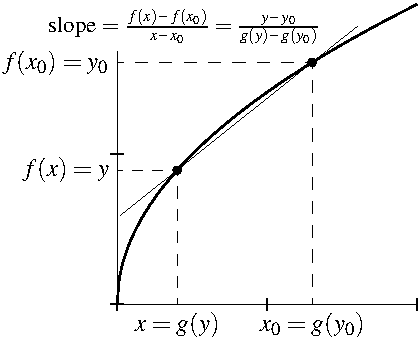
\includegraphics{figures/inversefigA}
\quad
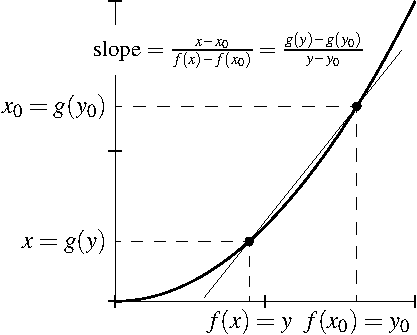
\includegraphics{figures/inversefigB}
\caption{Interpretation of the derivative of the inverse
function.\label{inversefig}}
\end{myfigureht}

Let
\begin{equation*}
Q(x) :=
\begin{cases}
\frac{x-x_0}{f(x)-f(x_0)} & \text{if $x \neq x_0$,} \\
\frac{1}{f'(x_0)} & \text{if $x = x_0$ (notice that $f'(x_0) \neq 0$).}
\end{cases}
\end{equation*}
As $f$ is differentiable at $x_0$, 
we have
\begin{equation*}
\lim_{x \to x_0} Q(x) =
\lim_{x \to x_0} 
\frac{x-x_0}{f(x)-f(x_0)} 
=
\frac{1}{f'(x_0)}
=
Q(x_0) ,
\end{equation*}
that is, $Q$ is continuous at $x_0$.
As $g(y)$ is continuous at $y_0$,
the composition $Q\bigl(g(y)\bigr) = \frac{g(y)-g(y_0)}{y-y_0}$
is continuous at $y_0$ by
\propref{prop:compositioncont}.
Therefore
\begin{equation*}
\frac{1}{f'\bigl(g(y_0)\bigr)}
= Q\bigl(g(y_0)\bigr)
= \lim_{y \to y_0} Q\bigl(g(y)\bigr)
= \lim_{y \to y_0} \frac{g(y)-g(y_0)}{y-y_0} .
\end{equation*}
So $g$ is differentiable at $y_0$ and $g'(y_0) =
\frac{1}{f'\left(\vphantom{1^1_1}g(y_0)\right)}$.

If $f'$ is continuous and nonzero at all $x \in I$,
then the lemma applies at all $x \in I$.  As $g$ is also
continuous, the derivative $g'(y) =
\frac{1}{f'\left(\vphantom{1^1_1}g(y)\right)}$ must be continuous.
\end{proof}

What is usually called the inverse function theorem is the following result.

\begin{thm}[Inverse function theorem]\index{inverse function theorem}
Let $f \colon (a,b) \to \R$ be a continuously differentiable function,
$x_0 \in (a,b)$ a point where $f'(x_0) \not= 0$.  Then there exists
an open interval $I \subset (a,b)$ with $x_0 \in I$, the
restriction $f|_{I}$ is injective with a continuously differentiable inverse
$g \colon J \to I$ defined on an interval $J := f(I)$,
and
\begin{equation*}
g'(y) = \frac{1}{f'\bigl( g(y) \bigr)} , \qquad \text{for all $y \in J$}.
\end{equation*}
\end{thm}

\begin{proof}
Without loss of generality, suppose $f'(x_0) > 0$.  As $f'$ is
continuous, there must exist an open interval $I = (x_0-\delta,x_0+\delta)$ 
such that $f'(x) > 0$ for all $x \in I$.  See
\exerciseref{exercise:positivecontneigh}.

By \propref{incdecdiffstrictprop} $f$ is strictly increasing
on $I$, and hence the restriction $f|_{I}$ bijective onto $J: = f(I)$.
As $f$ is continuous,
then by the
\corref{cor:continterval}
(or directly via the
\hyperref[IVT:thm]{intermediate value theorem})
$f(I)$ is in interval.
Now apply \lemmaref{lemma:ift}.
\end{proof}

If you tried to prove the existence of roots directly as in
\exampleref{example:sqrt2} you saw
how difficult that endeavor is.  However, with the machinery we have built
for inverse functions it becomes
an almost trivial exercise, and with the lemma above we prove
far more than mere existence.

\begin{cor}
Given any $n \in \N$ and any $x \geq 0$ there exists a unique 
number $y \geq 0$ (denoted $x^{1/n} := y$), such that $y^n = x$.  Furthermore,
the function $g \colon (0,\infty) \to (0,\infty)$ defined by
$g(x) := x^{1/n}$ is continuously differentiable and
\begin{equation*}
g'(x) = \frac{1}{nx^{(n-1)/n}} = \frac{1}{n} \, x^{(1-n)/n} ,
\end{equation*}
using the convention $x^{m/n} := {(x^{1/n})}^{m}$.
\end{cor}

\begin{proof}
For $x=0$ the existence of a unique root is trivial.

Let $f \colon (0,\infty) \to (0,\infty)$ be defined by $f(y) := y^n$.
The function $f$ is continuously differentiable
and $f'(y) = ny^{n-1}$, see \exerciseref{exercise:diffofxn}.  For $y > 0$ the derivative $f'$ is strictly positive
and so again by \propref{incdecdiffstrictprop}, $f$ is strictly
increasing (this can also be proved directly).
Given any $M > 1$, $f(M) = M^n \geq M$, and given any $1 > \epsilon > 0$,
$f(\epsilon) = \epsilon^n \leq \epsilon$.  For any $x$ with $\epsilon < x <
M$ we have by the
\hyperref[IVT:thm]{intermediate value theorem} that $x \in
f\bigl( [\epsilon,M] \bigr) \subset
f\bigl( (0,\infty) \bigr)$.  As $M$ and $\epsilon$ were arbitrary, $f$ is onto
$(0,\infty)$, and hence $f$ is bijective.
Let $g$ be the inverse of $f$ and we obtain
the existence and uniqueness of positive
$n$th roots.  \lemmaref{lemma:ift} says $g$ has a continuous
derivative and $g'(x) =
\frac{1}{f'\left(\vphantom{1^1_1}g(x)\right)} = \frac{1}{n {(x^{1/n})}^{n-1}}$.
\end{proof}

\begin{example}
The corollary provides a good example of where the inverse function theorem
gives us an interval smaller than $(a,b)$.  Take $f \colon \R \to \R$
defined by $f(x) := x^2$.  Then $f'(x) \not= 0$
as long as $x \not= 0$.  If $x_0 > 0$, we can take $I=(0,\infty)$, but
no larger.
\end{example}

\begin{example}
Another useful example is $f(x) := x^3$.  The function $f \colon \R \to \R$ is
one-to-one and onto, so $f^{-1}(y) = y^{1/3}$ exists on the entire real
line including zero and negative $y$.  The function $f$ has
a continuous derivative, but $f^{-1}$ has no derivative at the origin.  The
point is that $f'(0) = 0$.  See \figureref{cubecuberootfig} for a graph,
notice the vertical tangent on the cube root at the origin.
See also \exerciseref{exercise:oddroot}.
\begin{myfigureht}
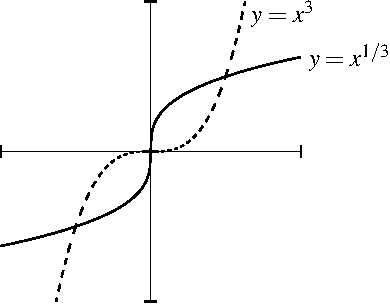
\includegraphics{figures/cubecuberoot}
\caption{Graphs of $x^3$ and $x^{1/3}$.\label{cubecuberootfig}}
\end{myfigureht}
\end{example}


\subsection{Exercises}

\begin{exercise}
Suppose $f \colon \R \to \R$ is continuously differentiable such that
$f'(x) > 0$ for all $x$.  Show that $f$ is invertible on the interval $J =
f(\R)$, the inverse is continuously differentiable, and ${(f^{-1})}'(y) >
0$ for all $y \in f(\R)$.
\end{exercise}

\begin{exercise}
Suppose $I,J$ are intervals and a monotone onto $f \colon I \to J$ has an inverse $g \colon J \to I$.
Suppose you already know that both $f$ and $g$ are differentiable
everywhere and $f'$ is never zero.  Using chain rule but not \lemmaref{lemma:ift} prove the
formula $g'(y) = \frac{1}{f'\left(\vphantom{1_1^1}g(y)\right)}$. % \bigl( \bigr) are overly big here!
\end{exercise}

\begin{exercise}
Let $n\in \N$ be even.
Prove that every $x > 0$ has a unique negative $n$th root.
That is, there exists a negative number $y$ such that $y^n = x$.
Compute the derivative
of the function $g(x) := y$.
\end{exercise}

\begin{exercise} \label{exercise:oddroot}
Let $n \in \N$ be odd and $n \geq 3$.
Prove that every $x$ has a unique $n$th root.
That is, there exists a number $y$ such that $y^n = x$.  Prove that
the function defined by $g(x) := y$ is differentiable except at $x=0$
and compute the derivative.  Prove that $g$ is not differentiable at $x=0$.
\end{exercise}

\begin{exercise}[requires \sectionref{sec:taylor}]
Show that if in the inverse function theorem $f$ has $k$ continuous
derivatives, then the inverse function $g$ also has $k$ continuous
derivatives.
\end{exercise}

\begin{exercise}
Let $f(x) := x + 2 x^2 \sin(\nicefrac{1}{x})$ for $x \not= 0$ and
$f(0) = 0$.  Show that $f$ is differentiable at all $x$, that $f'(0) > 0$,
but that $f$ is not invertible
on any open interval containing the origin.
\end{exercise}

\begin{exercise}
{\ }
\begin{enumerate}[a)]
\item
Let $f \colon \R \to \R$ be a continuously differentiable function
and $k > 0$ be a number such that $f'(x) \geq k$ for all $x \in \R$.
Show $f$ is one-to-one and onto, and has a continuously differentiable
inverse $f^{-1} \colon \R \to \R$.
\item
Find an example $f \colon \R \to \R$
where $f'(x) > 0$
for all $x$, but $f$ is not onto.
\end{enumerate}
\end{exercise}

\begin{exercise}
Suppose $I,J$ are intervals and a monotone onto $f \colon I \to J$ has an inverse $g \colon J \to I$.
Suppose $x \in I$ and $y := f(x) \in J$, and that $g$ is differentiable at
$y$.  Prove:
\begin{enumerate}[a)]
\item
If $g'(y) \not= 0$, then $f$ is differentiable at $x$.
\item
If $g'(y) = 0$, then $f$ is not differentiable at $x$.
\end{enumerate}
\end{exercise}
